\documentclass[11pt]{article}

\usepackage[margin=1in]{geometry}
\usepackage{amsmath}
\usepackage{amssymb}
\usepackage{booktabs}
\usepackage{graphicx}
\usepackage{microtype}
\usepackage{xcolor}
\usepackage[hidelinks]{hyperref}

\title{\textbf{Neural Firmware for Exact Integer Addition}\\
\large A Controlled Small-Transformer Study}
\author{Josiah Wilson\\Independent Researcher}
\date{July 26, 2026}

\begin{document}
\maketitle

\begin{abstract}
Autoregressive neural networks can imitate arithmetic procedures without
reliably preserving them outside the lengths represented in training. We test
a narrow alternative: place a known deterministic process inside the model's
forward path as immutable ``neural firmware,'' while leaving the surrounding
transformer trainable. A 264{,}480-parameter causal transformer was compared
with an otherwise identical model augmented by a frozen decimal ripple-carry
transducer. The transducer encoded the correct next answer token as a fixed
latent vector; the transformer's learned output head decoded that vector.
Models were trained on additions with one- to six-digit nonnegative operands.
In a preregistered confirmatory study using three unseen training seeds, the
generic transformer averaged \(90.13\%\) exact-match accuracy in range but
\(0\%\) on both 7--12 and 13--20 digit random additions. The latent-firmware
model achieved \(100\%\) on every split for every seed, including 10{,}500 of
10{,}500 confirmatory examples across its three runs. A direct-logit firmware
upper bound was also perfect. A post-hoc ablation that set firmware strength to
zero reduced the trained latent models to \(0\%\) on both extrapolation splits.
These results establish a limited engineering proposition: an exact process
can be installed as frozen computation and made usable through a learned
latent interface on a controlled grammar. They do not establish general
mathematical reasoning. The input parser and operation selection were fixed,
the baseline was not a task-specialized arithmetic transformer, and the
firmware was a PyTorch transition-table module rather than a program compiled
entirely into standard transformer weights.
\end{abstract}

\section{Introduction}

Language models generate sequences by learning statistical structure. This
makes them flexible, but it also asks gradient-based optimization to rediscover
procedures that are already known exactly. Arithmetic is a canonical example:
models can interpolate well over familiar operand lengths while failing
abruptly on longer inputs \cite{brown2020language,jelassi2023length}. Increasing
scale or arithmetic data can reduce errors without making addition
truth-preserving by construction.

An alternative is to separate uncertain inference from known computation.
When a process is already fully specified---integer addition, parsing a formal
grammar, applying a type rule, or advancing a board-game state---the process
need not be relearned as an approximation. It can instead be installed as
immutable computation and connected to a learned model at its boundaries. We
call such a component \emph{neural firmware}: fixed algorithmic structure
executed within a neural model's forward path.

This idea is adjacent to neural arithmetic modules
\cite{trask2018neural}, neural algorithmic reasoning
\cite{velickovic2021neural}, differentiable and neural compilation
\cite{bunel2016adaptive,saldyt2024algorithmic}, compiled transformers
\cite{lindner2023tracr,shaw2024alta}, and hybrid transformer--reasoner
architectures \cite{bounsi2024transformers}. Recent work has also translated
symbolic scientific programs into frozen differentiable PyTorch modules
\cite{sheneman2026compiler}. Our experiment is intentionally smaller. It asks
whether an immutable ripple-carry process can be injected into a compact
autoregressive transformer through a fixed latent code and remain exact when
the learned baseline leaves its training-length distribution.

The study makes three contributions:

\begin{enumerate}
    \item It implements a zero-trainable-parameter decimal ripple-carry module
    and integrates its outputs into the residual stream of a causal
    transformer.
    \item It evaluates the interface in a preregistered, multi-seed experiment
    with procedurally generated, held-out additions and adversarial carry
    chains.
    \item It documents an important boundary discovered during pilots:
    deterministic execution alone is insufficient if its latent signal can be
    overwhelmed by learned activations at unseen positions.
\end{enumerate}

The intended claim is narrow. This is a controlled proof of engineering
feasibility, not a demonstration that mathematical hallucination has been
solved.

\section{Related Work}

\subsection{Learning arithmetic algorithms}

Neural architectures have long been tested on arithmetic because algorithms
provide exact targets and clean extrapolation regimes. Neural GPUs learned
binary addition and multiplication on inputs longer than those in training
\cite{kaiser2015neural}, and later refinements learned decimal multiplication
\cite{freivalds2017improving}. Neural Arithmetic Logic Units introduced
architectural biases for additive and multiplicative extrapolation
\cite{trask2018neural}. These approaches seek learned mechanisms that behave
algorithmically.

Transformers can also length-generalize under carefully chosen inductive
biases. Relative positions can support addition beyond trained lengths
\cite{jelassi2023length}; position coupling aligns digits of equal significance
and has generalized from 30 to 200 digits \cite{cho2024position}; calibrated
attention biases and structured scratchpads provide additional routes
\cite{duan2023interpolation,cho2024arithmetic}. Consequently, the baseline in
this paper should not be interpreted as the strongest known arithmetic
transformer. It is a deliberately generic causal language-model architecture.
Our question differs: what happens when the known operation is specified and
frozen rather than induced?

\subsection{Neural compilation and hybrid reasoners}

Adaptive Neural Compilation showed that low-level programs can be mapped into
differentiable representations and subsequently optimized
\cite{bunel2016adaptive}. RASP supplied a programming abstraction for
transformer computation \cite{weiss2021thinking}, and Tracr compiled
human-readable RASP programs into standard decoder-only transformer weights
\cite{lindner2023tracr}. ALTA extended compiler-based analysis with loops and
Universal Transformers \cite{shaw2024alta}.

Several works move closer to language-model integration. Algorithmic Language
Models augment transformer architectures with memory, registers, basic
operations, and neurally compiled program libraries
\cite{saldyt2024algorithmic}. TransNAR combines transformer language
representations with frozen neural algorithmic reasoners
\cite{bounsi2024transformers}. Tracr-Injection distills compiled symbolic
variables into GPT-2 residual streams, but reports inconsistent
out-of-distribution generalization and \(95\%\) accuracy on its integer
addition experiment \cite{vergarabrowne2025tracr}. The Neural Compiler
translates first-order symbolic expressions into frozen differentiable modules
that match their source programs to floating-point precision
\cite{sheneman2026compiler}.

Our prototype sits between external tool use and full neural compilation. The
ripple-carry process is an \texttt{nn.Module} executed inside the forward path
and represented by immutable integer transition tables. It is not an external
calculator call, but it is also not yet compiled entirely into ordinary
attention and feed-forward weights.

The closest prior integrated-calculator work is Dietz and Klakow's Integrated
Gated Calculator (IGC) \cite{dietz2025igc}. IGC freezes Llama 3.1 8B and
trains learned input and output mappings around a non-differentiable
calculator, reporting 98--99\% on BIG-Bench Arithmetic across four
operations. It therefore predates this experiment as evidence for the broad
idea of an internally gated exact calculator. The present study is narrower:
a controlled small-transformer test of an immutable typed addition process,
multi-seed length extrapolation, and causal ablation. The studies use different
models, tasks, and interfaces and are not head-to-head.

\section{Method}

\subsection{Task and tokenizer}

Each sequence followed the grammar

\[
\texttt{<bos>}\;a\texttt{+}b\texttt{=}c\texttt{<eos>},
\qquad c=a+b,
\]

where \(a\) and \(b\) were nonnegative base-10 integers without leading zeros
except for zero itself. A transparent character tokenizer contained 15 symbols:
padding, beginning- and end-of-sequence symbols, ten digits, plus, and equals.
Loss was applied only to answer digits and the end token.

Training operand lengths were sampled independently and uniformly from one
through six digits. Training examples were generated online, eliminating
finite-dataset memorization and conventional benchmark contamination.

\subsection{Generic causal transformer}

All models shared the same trainable architecture:

\begin{itemize}
    \item three causal transformer encoder layers used as a decoder-only model;
    \item hidden width 96, four attention heads, and feed-forward width 256;
    \item fixed sinusoidal positions, zero dropout, and maximum sequence length
    96;
    \item an untied linear vocabulary head.
\end{itemize}

Each model contained 264{,}480 trainable parameters. Firmware buffers were not
counted as parameters.

\subsection{Frozen ripple-carry firmware}

The deterministic module stored two transition tables over
\((d_a,d_b,r)\in\{0,\dots,9\}^2\times\{0,1\}\):

\begin{align}
s(d_a,d_b,r) &= (d_a+d_b+r)\bmod 10,\\
r'(d_a,d_b,r) &= \left\lfloor\frac{d_a+d_b+r}{10}\right\rfloor.
\end{align}

Digits were processed from least to most significant and the resulting
sequence was reversed for normal left-to-right rendering. The tables were
registered buffers and the module exposed no trainable parameters. Unit tests
compared it with Python integer addition on 2{,}000 random pairs up to 20
digits.

The parser located the plus and equals tokens and extracted digit-token
operands. This parser was fixed and grammar-specific. The experiment therefore
does not test learned semantic parsing or learned operation selection.

\subsection{Latent and direct interfaces}

For each vocabulary item \(y\), a fixed random unit vector \(C[y]\in
\mathbb{R}^{96}\) was generated once using seed 314159. At a valid
answer-generation position \(t\), the latent-firmware model computed the exact
next token \(y_t^\star\) and modified the normalized transformer state:

\[
\widetilde{h}_t = h_t + \alpha C[y_t^\star],
\qquad \alpha=32.
\]

The ordinary trainable output head then produced logits from
\(\widetilde{h}_t\). Thus the deterministic module supplied exact content, but
the model still had to learn how the fixed latent code mapped to output tokens.

The direct-firmware upper bound added a large one-hot bias for
\(y_t^\star\) directly to the logits. It tested whether the transition process
and autoregressive alignment were exact independent of latent decoding.

Pilot experiments selected \(\alpha=32\) before confirmatory seeds or examples
were evaluated. At \(\alpha=8\), the model often terminated early at unseen
positions even though the ripple-carry output was correct. Signals of 20 or
more removed those pilot errors. This observation motivated the conservative
confirmatory strength of 32.

\subsection{Training}

AdamW used a learning rate of \(5\times10^{-4}\), weight decay 0.01, batch size
128, and gradient-norm clipping at 1.0. The generic baseline received 10{,}000
steps because pilots showed that it required that budget to exceed \(90\%\)
in-range exact match. The latent interface converged within 1{,}000 steps and
received 1{,}000 confirmatory steps. The direct upper bound received one step
because its result was structural, not learned. Giving the baseline ten times
more optimization steps makes the accuracy comparison conservative, but
prevents wall time from being interpreted as a controlled efficiency result.

\subsection{Preregistration and evaluation}

Pilot observations, decisions, and the confirmatory configuration were
committed before confirmatory execution. Confirmatory training seeds were 101,
211, and 307; none appeared in pilots. Evaluation used the unseen seed 918273.
All models were evaluated on the same committed examples:

\begin{itemize}
    \item \textbf{ID random}: 1{,}000 additions with one- to six-digit operands;
    \item \textbf{OOD primary}: 1{,}000 additions with 7--12 digit operands;
    \item \textbf{OOD long}: 1{,}000 additions with 13--20 digit operands;
    \item \textbf{carry chain}: 500 constructed additions dominated by long
    runs of trailing nines.
\end{itemize}

The primary outcome was sequence-level exact-match accuracy on OOD primary,
aggregated across the three training seeds. The logical evaluation-set hash was
\texttt{917935e56a1d\ldots23bd9b}; the full value appears in the appendix.

Experiments ran locally on an Apple M4 Mac mini with a 10-core GPU and 16 GB
unified memory, using Python 3.12.12 and PyTorch 2.13.0 on MPS.

\section{Results}

\subsection{Confirmatory accuracy}

Table~\ref{tab:main-results} reports mean exact-match accuracy over three
training seeds. The generic baseline learned the trained range, averaging
\(90.13\%\), but produced no correct answers on either random extrapolation
split. It solved one of 1{,}500 carry-chain cases across all seeds. Both
firmware interfaces were perfect on every confirmatory example.

\begin{table}[ht]
\centering
\caption{Exact-match accuracy, mean \(\pm\) sample standard deviation across
three training seeds.}
\label{tab:main-results}
\begin{tabular}{lcccc}
\toprule
Model & ID 1--6 & OOD 7--12 & OOD 13--20 & Carry chain\\
\midrule
Baseline & \(0.9013\pm0.0145\) & \(0.0000\pm0.0000\) &
\(0.0000\pm0.0000\) & \(0.0007\pm0.0012\)\\
Latent firmware & \(1.0000\pm0.0000\) & \(1.0000\pm0.0000\) &
\(1.0000\pm0.0000\) & \(1.0000\pm0.0000\)\\
Direct firmware & \(1.0000\pm0.0000\) & \(1.0000\pm0.0000\) &
\(1.0000\pm0.0000\) & \(1.0000\pm0.0000\)\\
\bottomrule
\end{tabular}
\end{table}

\begin{figure}[ht]
\centering
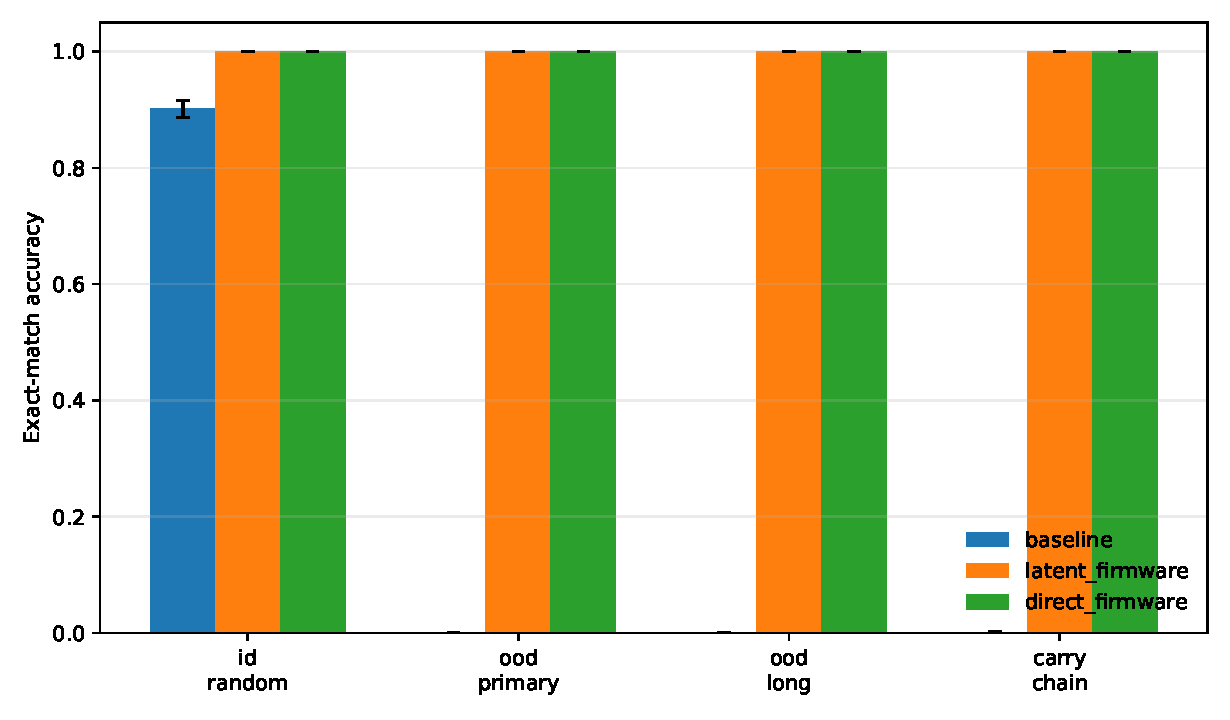
\includegraphics[width=\linewidth]{../figures/accuracy_by_split.pdf}
\caption{Exact-match accuracy by evaluation split. Error bars show standard
deviation across three training seeds.}
\label{fig:split}
\end{figure}

The primary latent-minus-baseline difference was 1.000 for each training seed,
or 100 percentage points. A bootstrap over the three seed-level differences
therefore returned a degenerate 95\% interval of [1.000, 1.000]. This interval
describes these seeds only; three seeds are insufficient for a broad claim
about optimization variability.

Across its three runs, latent firmware answered 10{,}500 of 10{,}500
confirmatory examples correctly. The baselines answered 2{,}704 of 3{,}000
in-range examples, zero of 6{,}000 random extrapolation examples, and one of
1{,}500 carry-chain examples.

\begin{figure}[ht]
\centering
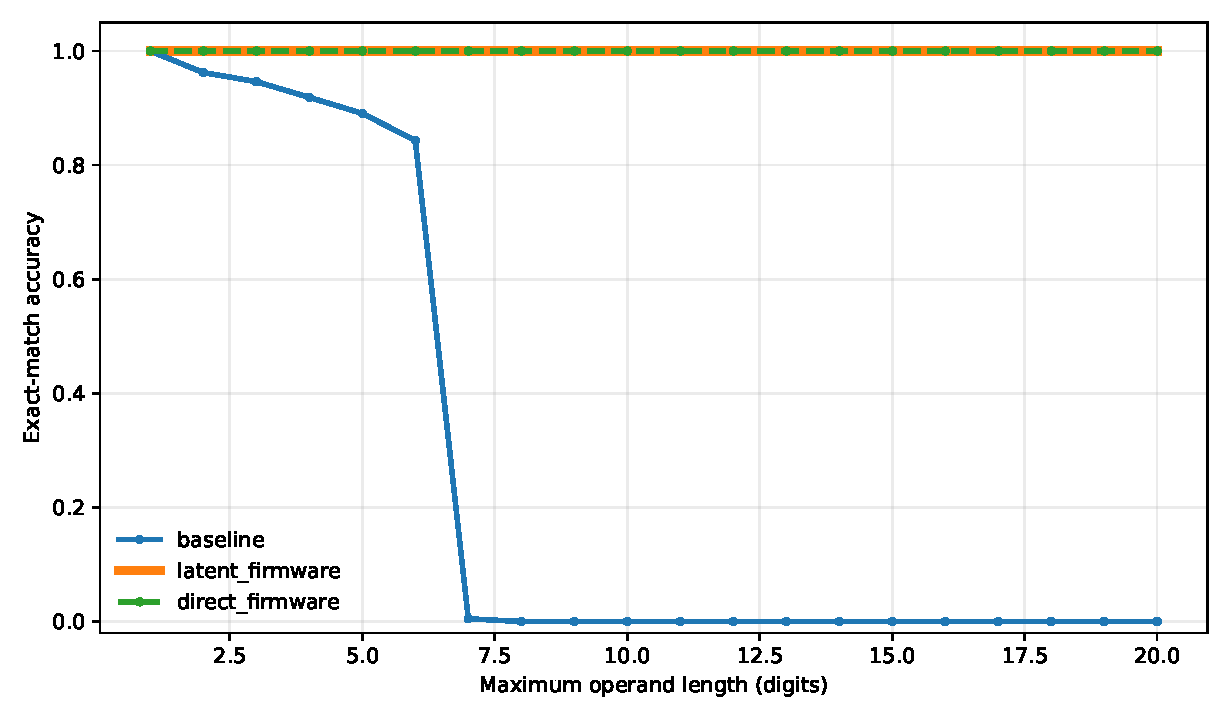
\includegraphics[width=\linewidth]{../figures/accuracy_by_digits.pdf}
\caption{Accuracy grouped by maximum operand length. The generic transformer's
performance drops sharply immediately beyond the six-digit training boundary;
both firmware paths remain exact through 20 digits.}
\label{fig:length}
\end{figure}

\subsection{Optimization and parameter counts}

Every variant had 264{,}480 trainable parameters. Table~\ref{tab:training}
reports observed training time. Because the step budgets were intentionally
different and the Python firmware parser added overhead, these numbers do not
constitute an efficiency comparison.

\begin{table}[ht]
\centering
\caption{Training budget and mean wall time over three seeds.}
\label{tab:training}
\begin{tabular}{lrrr}
\toprule
Model & Steps & Trainable parameters & Mean wall time\\
\midrule
Baseline & 10{,}000 & 264{,}480 & 689.8 s\\
Latent firmware & 1{,}000 & 264{,}480 & 224.5 s\\
Direct firmware & 1 & 264{,}480 & 0.17 s\\
\bottomrule
\end{tabular}
\end{table}

\subsection{Post-hoc firmware ablation}

After confirmatory analysis, firmware strength was set to zero without
retraining the three latent models. This was not preregistered and is reported
as a post-hoc causal check. In-range exact match fell to 0.2\%, 0.4\%, and
0.1\%; every model scored 0\% on OOD primary, OOD long, and carry chains.
Thus the confirmatory performance depended on the injected signal rather than
an arithmetic algorithm learned incidentally during the 1{,}000 interface
steps.

\section{Discussion}

\subsection{What the experiment establishes}

The study supports a limited proposition: exact algorithmic content can be
computed by an immutable module, encoded in a fixed latent subspace, and
decoded by a small generative transformer across sequence lengths not
represented in training. The trainable model did not need to rediscover
ripple-carry addition. It learned an interface to a process whose behavior was
specified.

The pilot strength failure is equally informative. A deterministic component
does not automatically make the hybrid system deterministic. At insufficient
signal strength, the learned residual stream overrode the correct latent code
at unfamiliar positions and caused premature termination. Reliability belongs
to the entire path:

\[
P(\text{correct}) =
P(\text{parse})\,
P(\text{route})\,
P(\text{execute})\,
P(\text{decode}).
\]

This experiment made execution exact and parsing trivial, then tuned the
decoding interface until it was reliable over the tested domain. Open-ended
mathematics would restore difficult parse and routing terms.

\subsection{Why this is not yet mathematical reliability}

The model never decided whether addition was appropriate. It received a narrow
formal grammar, and a fixed parser extracted the operands. A natural-language
word problem could still be formalized incorrectly and then computed perfectly.
Likewise, subtraction, multiplication, algebra, units, proof, and uncertainty
were not tested.

The observed exactness is empirical over bounded inputs, not a formal
end-to-end guarantee. The ripple-carry transition table is exact for valid
decimal tokens, but the full implementation includes an autoregressive decoder,
finite context, and software execution. ``Always mathematically correct'' would
require typed interfaces, validated routing, explicit preconditions, and
possibly proof-carrying outputs.

\subsection{Comparison with learned arithmetic methods}

The baseline uses fixed sinusoidal positions and ordinary causal attention.
Specialized architectures can learn length-generalizing addition
\cite{jelassi2023length,cho2024position,duan2023interpolation}. Therefore,
Figure~\ref{fig:length} is evidence against this generic baseline, not against
all learned arithmetic systems.

The distinction is architectural rather than leaderboard-oriented. A learned
method may achieve excellent empirical extrapolation and adapt to new
operations; a frozen process can preserve a known invariant by construction
but needs an explicit representation and interface. A useful future system may
combine both: learned decomposition and routing around a library of exact
typed primitives.

\section{Limitations}

\begin{enumerate}
    \item \textbf{Fixed formalization.} Parsing and operation selection were
    deterministic. The experiment does not test natural language.
    \item \textbf{Not compiled into standard transformer weights.} The
    firmware is a PyTorch module using integer tables and Python control flow.
    Calling it ``neural firmware'' describes architectural placement and latent
    integration, not a claim that ripple-carry addition emerged entirely from
    dense neural weights.
    \item \textbf{Generic baseline.} No relative-position, position-coupled,
    scratchpad, Neural GPU, or NALU baseline was implemented.
    \item \textbf{Single operation and number system.} Only nonnegative
    base-10 addition was evaluated.
    \item \textbf{Bounded evaluation.} Operands ended at 20 digits and sequences
    at 96 tokens.
    \item \textbf{No retained general language capability.} The small model was
    trained only on the controlled arithmetic grammar.
    \item \textbf{Three training seeds.} Replication was exact across all
    seeds, but the seed-level sample is small.
    \item \textbf{Unequal training budgets.} The baseline received ten times
    more steps; this is conservative for accuracy but prevents an efficiency
    comparison.
\end{enumerate}

\section{Next Experiments}

The next study should move one boundary at a time:

\begin{enumerate}
    \item compile the ripple-carry program into frozen tensor operations or
    transformer weights using a Tracr- or ALTA-like path;
    \item replace the fixed grammar parser with a supervised typed encoder and
    measure parse, route, execute, and decode failures separately;
    \item introduce several operations and a learned hard router, including
    malformed-input rejection;
    \item inject the subsystem into a pretrained 100--500M parameter language
    model and measure general-language retention;
    \item compare with strong learned arithmetic baselines such as position
    coupling;
    \item extend the same architecture to stateful deterministic systems,
    including board-game transition rules and programming-language type
    constraints.
\end{enumerate}

\section{Conclusion}

A compact transformer trained to imitate addition generalized poorly beyond
its training-length boundary. The same trainable architecture, given an
immutable ripple-carry process through a sufficiently strong fixed latent code,
was exact across every tested length and seed. This does not solve mathematical
reasoning, but it validates the first architectural step: known deterministic
processes can be treated as internal computational structure rather than facts
that gradient descent must repeatedly approximate. It does not establish the
first integrated calculator in a language model; IGC is direct prior art. Its
contribution is the controlled small-transformer evidence and exact
out-of-range comparison reported here.

\section*{Acknowledgments and Attribution}

Josiah Wilson originated the research hypothesis: deterministic processes
could be installed as locked components inside generative neural models, with
mathematics serving as the first controlled test. OpenAI Codex assisted with
literature discovery, experimental design, implementation, execution,
analysis, visualization, and manuscript drafting under Wilson's direction.
All claims in this report are limited to the committed artifacts and observed
results.

\begin{thebibliography}{99}

\bibitem{brown2020language}
T.~B. Brown et al.
\newblock Language models are few-shot learners.
\newblock \emph{Advances in Neural Information Processing Systems},
33:1877--1901, 2020.
\newblock \url{https://arxiv.org/abs/2005.14165}.

\bibitem{kaiser2015neural}
L.~Kaiser and I.~Sutskever.
\newblock Neural GPUs learn algorithms.
\newblock arXiv:1511.08228, 2015.
\newblock \url{https://arxiv.org/abs/1511.08228}.

\bibitem{freivalds2017improving}
K.~Freivalds and R.~Liepins.
\newblock Improving the Neural GPU architecture for algorithm learning.
\newblock arXiv:1702.08727, 2017.
\newblock \url{https://arxiv.org/abs/1702.08727}.

\bibitem{trask2018neural}
A.~Trask, F.~Hill, S.~Reed, J.~Rae, C.~Dyer, and P.~Blunsom.
\newblock Neural arithmetic logic units.
\newblock \emph{Advances in Neural Information Processing Systems}, 31, 2018.
\newblock \url{https://arxiv.org/abs/1808.00508}.

\bibitem{bunel2016adaptive}
R.~R. Bunel, A.~Desmaison, P.~K. Mudigonda, P.~Kohli, and P.~H.~S. Torr.
\newblock Adaptive neural compilation.
\newblock \emph{Advances in Neural Information Processing Systems}, 29, 2016.
\newblock \url{https://arxiv.org/abs/1605.07969}.

\bibitem{velickovic2021neural}
P.~Velickovic and C.~Blundell.
\newblock Neural algorithmic reasoning.
\newblock \emph{Patterns}, 2(7):100273, 2021.
\newblock \url{https://arxiv.org/abs/2105.02761}.

\bibitem{weiss2021thinking}
G.~Weiss, Y.~Goldberg, and E.~Yahav.
\newblock Thinking like transformers.
\newblock In \emph{Proceedings of the 38th International Conference on Machine
Learning}, 2021.
\newblock \url{https://arxiv.org/abs/2106.06981}.

\bibitem{lindner2023tracr}
D.~Lindner, J.~Kramar, S.~Farquhar, M.~Rahtz, T.~McGrath, and V.~Mikulik.
\newblock Tracr: Compiled transformers as a laboratory for interpretability.
\newblock \emph{Advances in Neural Information Processing Systems}, 36, 2023.
\newblock \url{https://arxiv.org/abs/2301.05062}.

\bibitem{shaw2024alta}
P.~Shaw, J.~Cohan, J.~Eisenstein, K.~Lee, J.~Berant, and K.~Toutanova.
\newblock ALTA: Compiler-based analysis of transformers.
\newblock arXiv:2410.18077, 2024.
\newblock \url{https://arxiv.org/abs/2410.18077}.

\bibitem{saldyt2024algorithmic}
L.~Saldyt and S.~Kambhampati.
\newblock Algorithmic language models with neurally compiled libraries.
\newblock arXiv:2407.04899, 2024.
\newblock \url{https://arxiv.org/abs/2407.04899}.

\bibitem{bounsi2024transformers}
W.~Bounsi, B.~Ibarz, A.~Dudzik, J.~B. Hamrick, L.~Markeeva, A.~Vitvitskyi,
R.~Pascanu, and P.~Velickovic.
\newblock Transformers meet neural algorithmic reasoners.
\newblock arXiv:2406.09308, 2024.
\newblock \url{https://arxiv.org/abs/2406.09308}.

\bibitem{jelassi2023length}
S.~Jelassi, S.~d'Ascoli, C.~Domingo-Enrich, Y.~Wu, Y.~Li, and F.~Charton.
\newblock Length generalization in arithmetic transformers.
\newblock arXiv:2306.15400, 2023.
\newblock \url{https://arxiv.org/abs/2306.15400}.

\bibitem{cho2024position}
H.~Cho, J.~Cha, P.~Awasthi, S.~Bhojanapalli, A.~Gupta, and C.~Yun.
\newblock Position coupling: Improving length generalization of arithmetic
transformers using task structure.
\newblock arXiv:2405.20671, 2024.
\newblock \url{https://arxiv.org/abs/2405.20671}.

\bibitem{cho2024arithmetic}
H.~Cho, J.~Cha, S.~Bhojanapalli, and C.~Yun.
\newblock Arithmetic transformers can length-generalize in both operand length
and count.
\newblock arXiv:2410.15787, 2024.
\newblock \url{https://arxiv.org/abs/2410.15787}.

\bibitem{duan2023interpolation}
S.~Duan, Y.~Shi, and W.~Xu.
\newblock From interpolation to extrapolation: Complete length generalization
for arithmetic transformers.
\newblock arXiv:2310.11984, 2023.
\newblock \url{https://arxiv.org/abs/2310.11984}.

\bibitem{vergarabrowne2025tracr}
T.~Vergara-Browne and A.~Soto.
\newblock Tracr-Injection: Distilling algorithms into pre-trained language
models.
\newblock arXiv:2505.10719, 2025.
\newblock \url{https://arxiv.org/abs/2505.10719}.

\bibitem{sheneman2026compiler}
L.~Sheneman.
\newblock The Neural Compiler: Program-to-network translation for hybrid
scientific machine learning.
\newblock arXiv:2605.22498, 2026.
\newblock \url{https://arxiv.org/abs/2605.22498}.

\bibitem{dietz2025igc}
F.~Dietz and D.~Klakow.
\newblock IGC: Integrating a Gated Calculator into an LLM to Solve Arithmetic
Tasks Reliably and Efficiently.
\newblock 2025.
\newblock \url{https://arxiv.org/abs/2501.00684}.

\end{thebibliography}

\appendix

\section{Reproducibility Checklist}

\begin{itemize}
    \item Frozen confirmatory configuration:
    \texttt{configs/study.json}.
    \item Configuration commit:
    \texttt{22f1649e28079ce28620ac8c01b774d8009231cd}.
    \item Configuration SHA-256:
    {\scriptsize\texttt{6a2d375e789f6eaabc5cfa5d295ab9eb6752e040afe25aaf357b9425f29b33c1}}.
    \item Evaluation logical SHA-256:
    {\scriptsize\texttt{917935e56a1d1aecf72589c11721a695f1092066c9b97b875e1a49622393bd9b}}.
    \item Environment lock: \texttt{uv.lock}.
    \item Unit tests: eight passing tests at confirmatory execution.
    \item Compact run manifests, errors, summaries, and figures:
    \texttt{results/} and \texttt{figures/}.
\end{itemize}

Core reproduction commands:

\begin{verbatim}
uv sync --extra dev
uv run pytest
uv run nf-study --config configs/study.json
uv run nf-analyze \
  --study artifacts/confirmatory_v1/study.json
\end{verbatim}

\section{Pilot-to-Confirmatory Separation}

Pilots used training seed 17 and evaluation seed 260725. The initial latent
strength of 8 decoded correctly in distribution but failed at unseen
positions. A pilot-only sweep established that strengths of 20 or more removed
observed truncation. The final strength of 32 was frozen before confirmatory
training. Confirmatory seeds 101, 211, and 307 and evaluation seed 918273 were
not used during tuning. The complete chronological record is in
\texttt{PILOT\_LOG.md}.

\paragraph{Artifact scope.}
Large model checkpoints and full per-example predictions are retained locally
under ignored artifact directories. The Git-tracked artifact contains compact
study manifests, every baseline error, aggregate tables, environment records,
source code, configuration, figures, and this manuscript.

\end{document}
